 \documentclass{beamer}
\usepackage[english]{babel}
\usepackage{graphicx}
\usepackage{tcolorbox}
\usepackage{subfig}
\usepackage{booktabs}
\usepackage{multirow}
\usepackage{multicol}
\usepackage{physymb}
\usepackage{amsmath}
\usepackage{setspace}

\hypersetup{colorlinks,linkcolor=blue,urlcolor=blue}

\newcommand{\refsearsa}{Sears y Zemansky, 2013}
\newcommand{\refsearsb}{adaptada de Sears y Zemansky, 2013}
\newcommand*\diff{\mathop{}\!\mathrm{d}}
\newcommand*\Diff[1]{\mathop{}\!\mathrm{d^#1}}
\newcommand{\citetalk}[1]{ { \tiny { \begin{spacing}{0.75} #1 \end{spacing} } } }

\hypersetup{colorlinks=true,citecolor=blue,linkcolor=blue,urlcolor=blue}
\usetheme{CambridgeUS}
\usecolortheme{beaver}
\setbeamercolor{titlelike}{parent=structure,fg=white,bg=red}
\useoutertheme{smoothbars}
\useinnertheme{circles}

\beamertemplatenavigationsymbolsempty

\title[CONCAPAN]{ Espectroscopia óptica y computacional en estudios de la calidad del agua }
\author[Lic. J. Cuadra]{
\tiny{
\underline{J. Cuadra}, M. Ramos, S. de La O, N. Cisneros, O. Deodanes and C. Rudamas
}
}
\institute[UES]{
\tiny{
\inst{} Laboratorio de espectroscopia óptica, Escuela de Física, Facultad de Ciencias Naturales y Matemática, Universidad de El Salvador, Central America. 
\and  
\href{mailto://jorge.cuadra@ues.edu.sv}{jorge.cuadra@ues.edu.sv} \hspace{0.25cm} , \hspace{0.25cm} \href{mailto://carlos.rudamas@ues.edu.sv}{carlos.rudamas@ues.edu.sv}
}
}
\date{ \tiny{ \today } }

\AtBeginSection{ 
\begin{frame}
\frametitle{Contents}
\tableofcontents[currentsection]
\end{frame}
}

\AtBeginSubsection{ 
\begin{frame}
\frametitle{Contents}\section{Introduction}
\tableofcontents[currentsection,currentsubsection]
\end{frame}
}

%\pause

%\logo{
\includegraphics[scale=0.05]{Figures/Logo_UES.png}}

\begin{document}
	
\begin{frame}
\begin{center}
Foro: Aplicaciones medioambientales de la computación de alto rendimiento (HPC) y la espectroscopia óptica en Centroamérica
\end{center}
\titlepage

\includegraphics[scale=0.025]{Figures/Logo_UES.png}
\hspace{9.5cm}
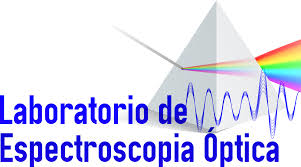
\includegraphics[scale=0.5]{Figures/Logo_LEO.png}
\end{frame}

\begin{frame}
%\frametitle{Contenido}
\tableofcontents
\end{frame}

\section{Introduction}

\begin{frame}
\frametitle{Water pollution problems}
\begin{columns}
\begin{column}{0.65\textwidth}
\begin{figure}

\includegraphics[scale=0.75]{./Figures/ONU_Goals.png}
\caption{ONU sustainable development goals}
\end{figure}
\end{column}
\begin{column}{0.35\textwidth}
\begin{itemize}
\item $^{\dotplus}$ 0.8 M early deaths associated to this type of pollution
\item $^{\dotplus}$ 1.4\% to 2.5\% of GDP investment due to water pollution
\item $^{\dagger, \dagger\dagger}$ Aguas superficiales contaminadas en El Salvador 
\end{itemize}
\end{column}
\end{columns}
\citetalk{$\dotplus$ Cost of Environmental Degradation: Air and Water Pollution, World Bank Group, 2021 }
\citetalk{$\dagger$ Autoridad Salvadoreña del Agua (ASA), laboratorio de calidad del agua, informe 2020}
\citetalk{ $\dagger\dagger$ Organización Panamericana de la Salud (OPS) y Organización Mundial de la Salud (OMS), Evaluación del sector agua potable y saneamiento en El Salvador; informe preliminar }
\end{frame}

\section{Measurements and Simulations}

\begin{frame}
\frametitle{Measurement place}
\begin{figure}
\centering
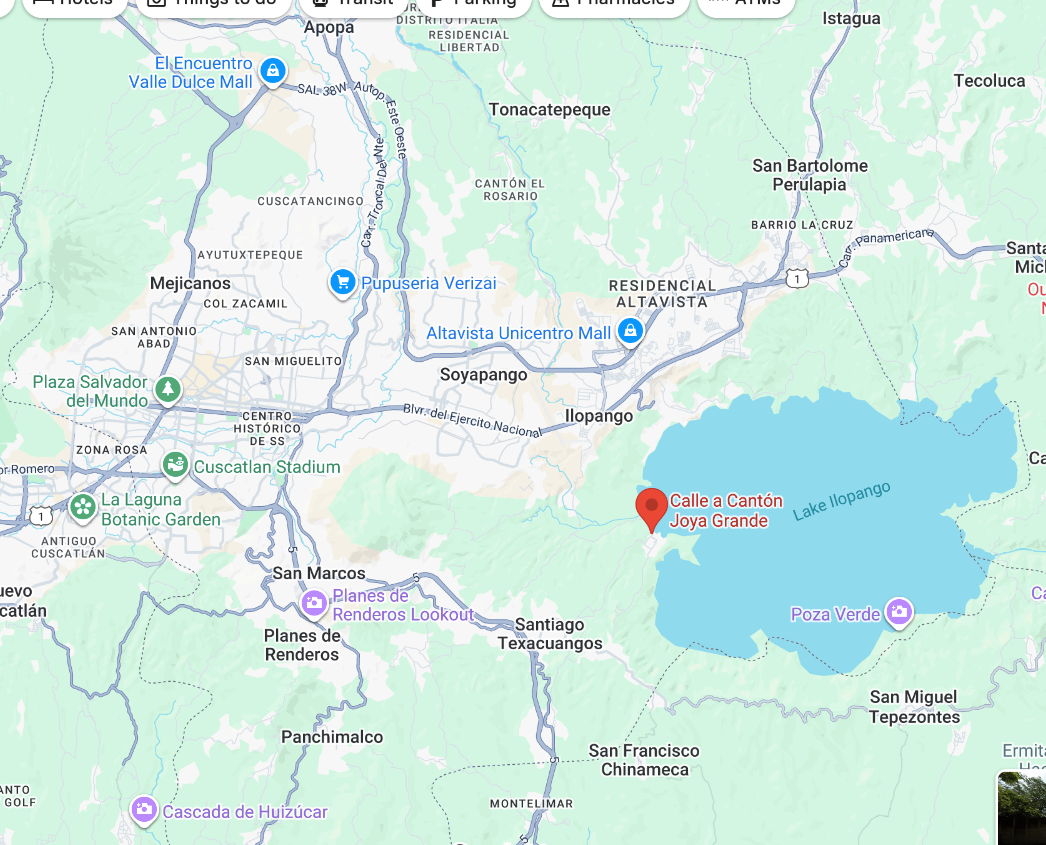
\includegraphics[scale=0.20]{./Figures/Measurement_Place2.png}
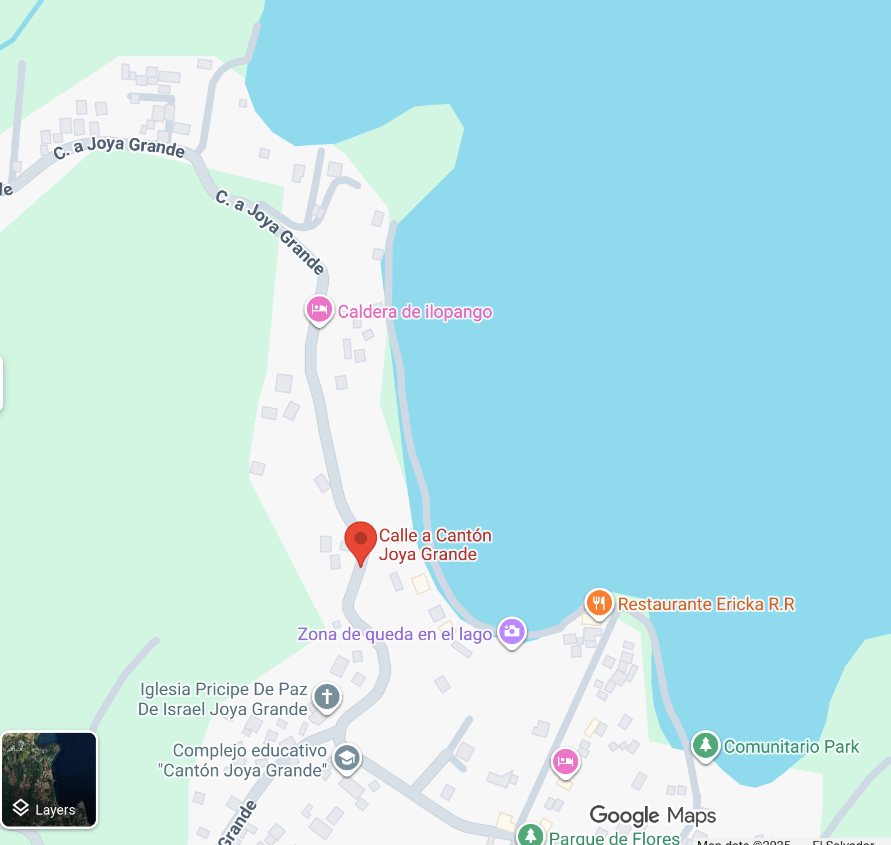
\includegraphics[scale=0.20]{./Figures/Measurement_Place1.png}
\caption{Cantón Joya Grande, Ilopango lake in map$^{\dagger}$.}
\end{figure}
\citetalk{$\dagger$Screenshot taken with Google Maps.}
\end{frame}

\begin{frame}
\frametitle{Measurements - conventional setup} 
\begin{columns}
\begin{column}{0.5\textwidth}
\begin{figure}
\centering
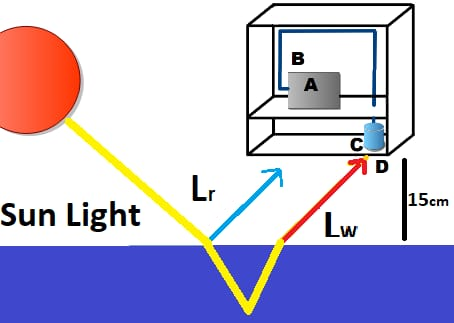
\includegraphics[scale=0.30]{./Figures/Setup_Conventional.jpeg}
\caption{Diagram for conventional reflectance measurement.}
\end{figure}
\end{column}
\begin{column}{0.5\textwidth}
\begin{figure}
\centering
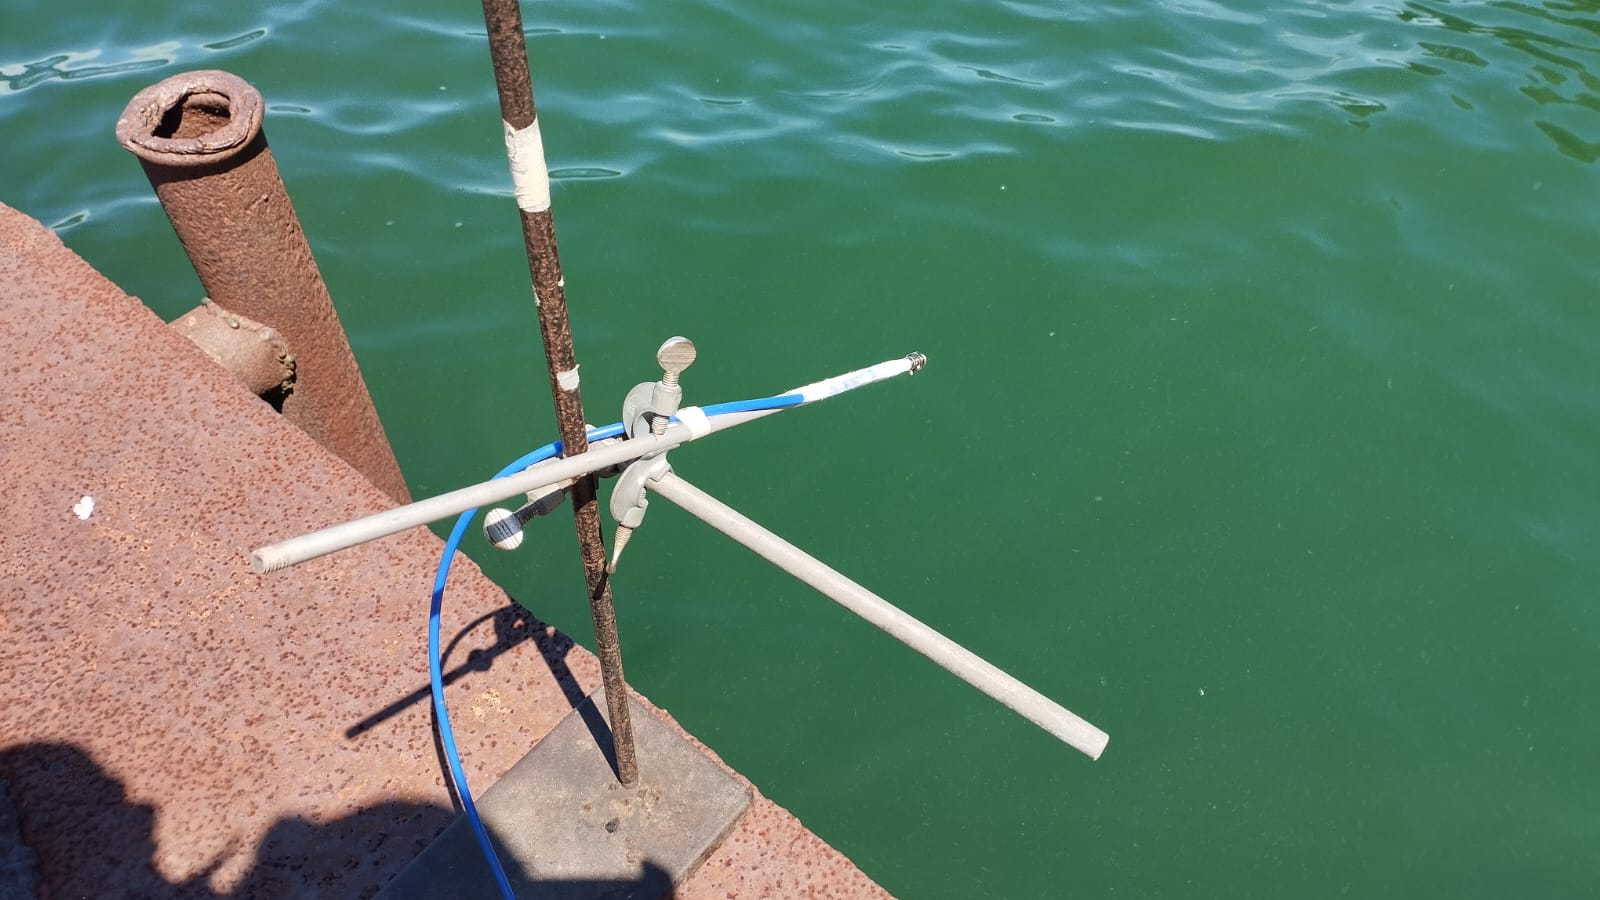
\includegraphics[scale=0.10]{./Figures/R_Conventional.jpeg}
\caption{Conventional Reflectance setup for water quality measurement.}
\end{figure}
\end{column}
\end{columns}
\end{frame}

\begin{frame}
\frametitle{Measurements - MA\&Z-DOAS prototype} 
\begin{columns}
\begin{column}{0.5\textwidth}
\begin{figure}
\centering
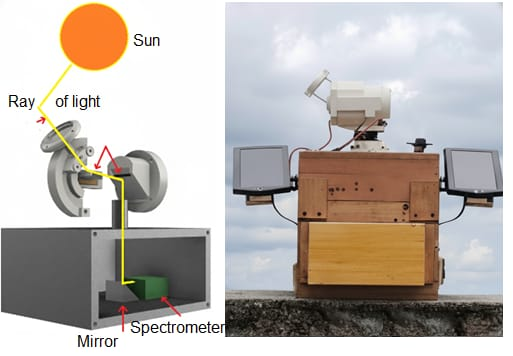
\includegraphics[scale=0.35]{./Figures/MAiZDOAS_Setup.jpeg}
\caption{Diagram for MA\&Z-DOAs measurement.}
\end{figure}
\end{column}
\begin{column}{0.5\textwidth}
\begin{figure}
\centering
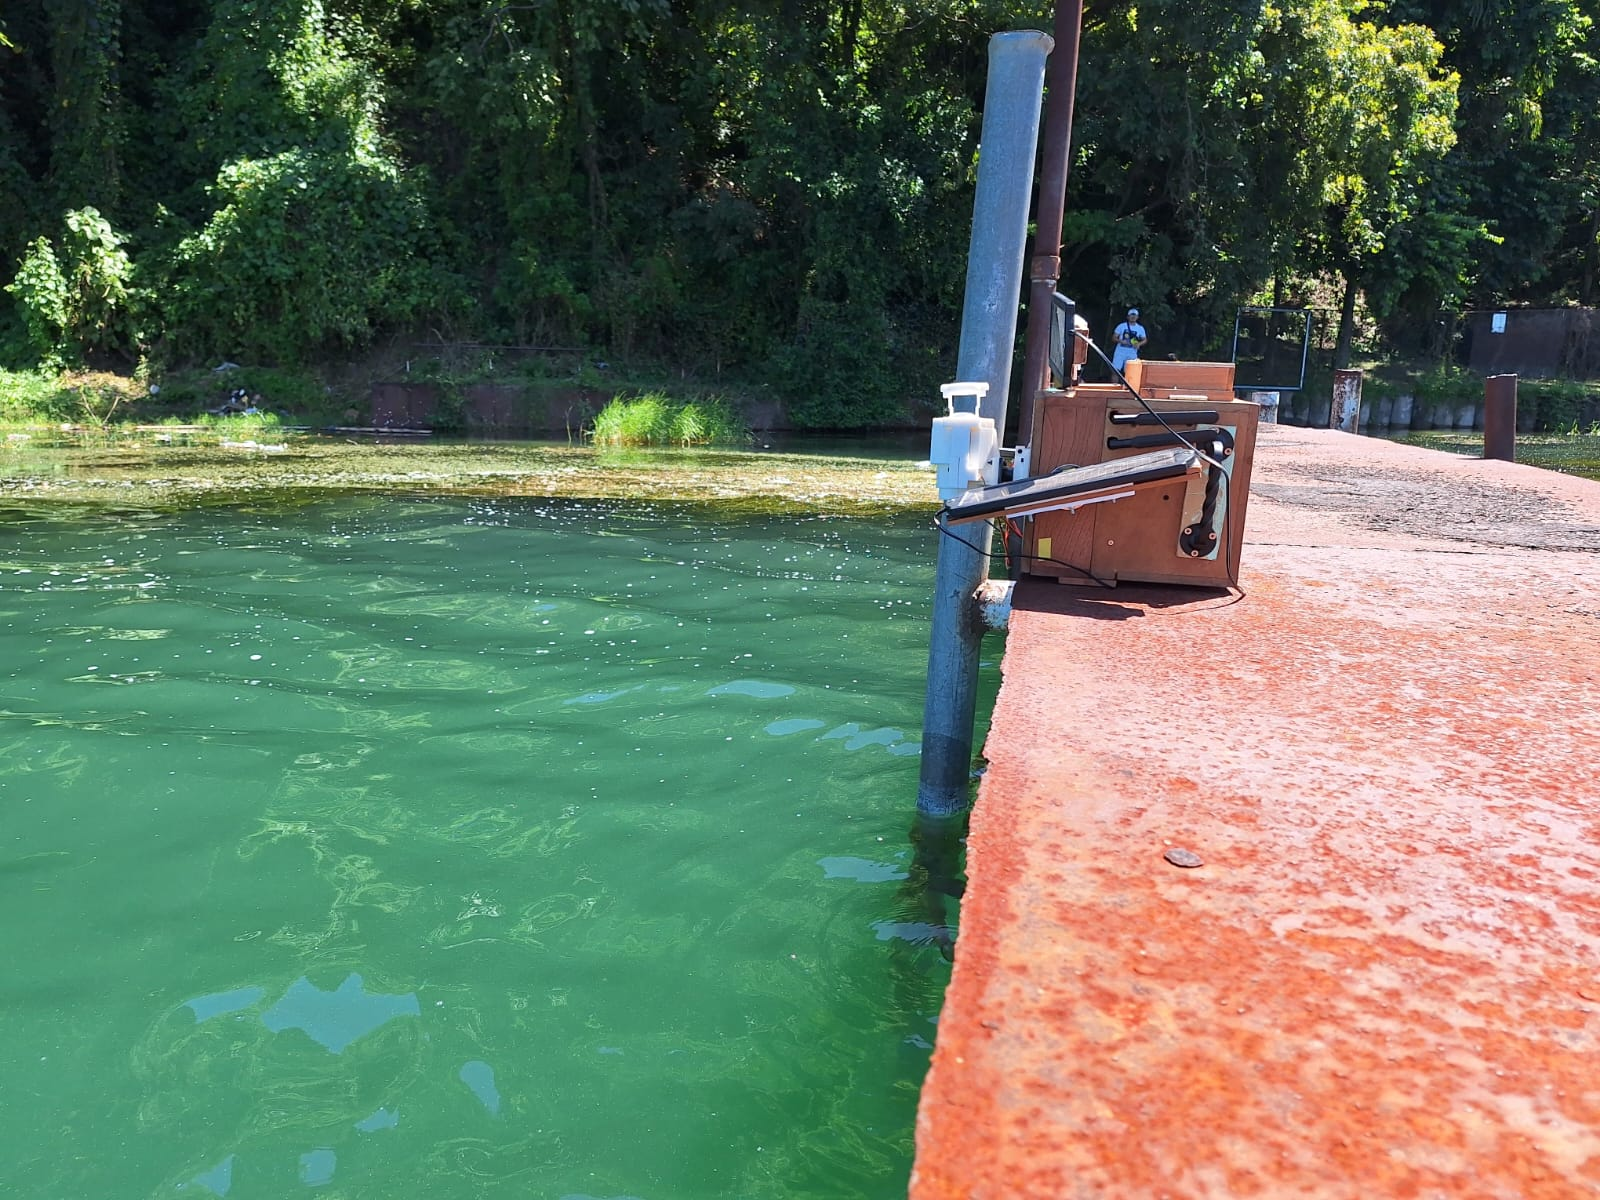
\includegraphics[scale=0.10]{./Figures/MAiZDOAS_WQ2.jpeg}
\caption{Conventional Reflectance setup for water quality measurement.}
\end{figure}
\end{column}
\end{columns}
\end{frame}

\begin{frame}
\frametitle{Reflectance model for remote sensing}
\begin{columns}
\begin{column}{0.5\textwidth}
\begin{figure}
\centering
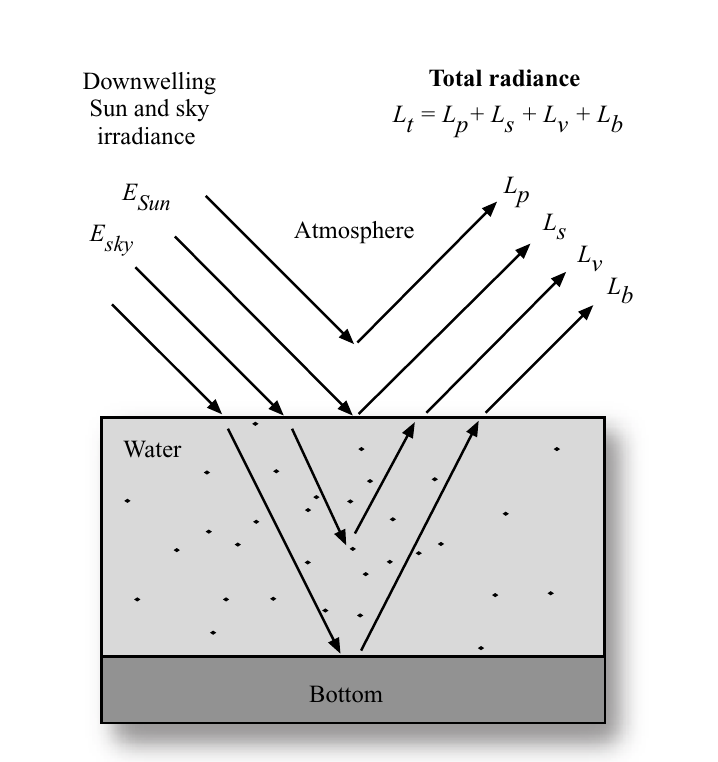
\includegraphics[scale=0.25]{./Figures/Jensen_2007.png}
\caption{Diagram of reflected irradiance in a body of water$\dagger$}
\end{figure}
\end{column}
\begin{column}{0.5\textwidth}
\begin{eqnarray}
R_{S} \left( \lambda \right) &=& \rho_{ls} \frac{ L_{t} \left( \lambda \right) }{ E_{t} \left( \lambda \right) }
\end{eqnarray}
\end{column}
\end{columns}
\citetalk{$\dagger$Jensen, J.R. (2007) Remote Sensing of the Environment: An Earth Resource Perspective. 2nd Edition, Pearson Prentice Hall, Upper Saddle River.}
\end{frame}

\begin{frame}
\frametitle{Low altitude and Shallow waters approximations}
\begin{columns}
\begin{column}{0.5\textwidth}
\begin{figure}
\centering
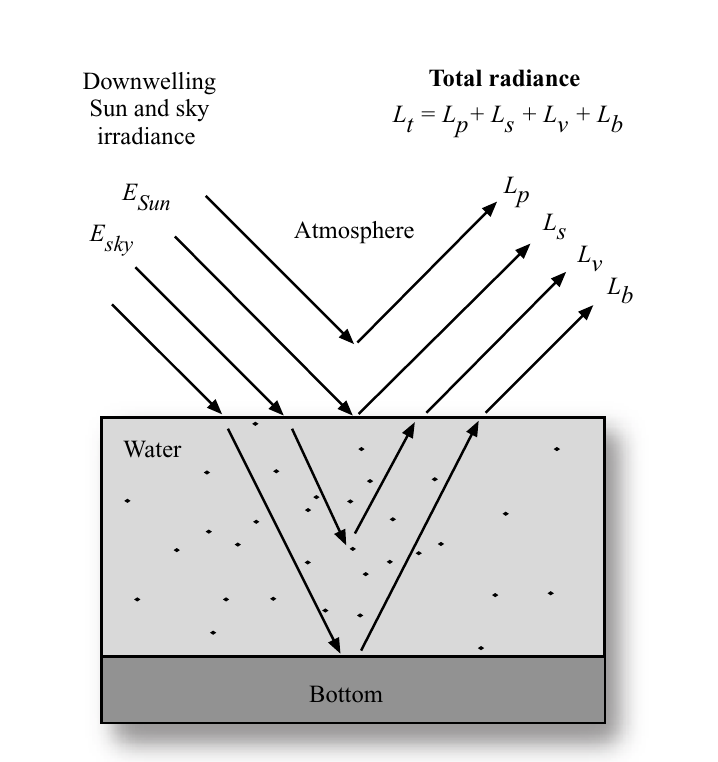
\includegraphics[scale=0.25]{./Figures/Jensen_2007.png}
\caption{Diagram of reflected irradiance in a body of water$\dagger$}
\end{figure}
\end{column}
\begin{column}{0.5\textwidth}
Approximation low altitude:
\begin{eqnarray}
E_{\mathrm{sky}} & \approx & 0 \nonumber \\
L_{\mathrm{p}} & \approx & 0 \nonumber
\end{eqnarray}
Approximation due to shallow waters:
\begin{eqnarray}
L_{S} & \approx & L_{V} \nonumber
\end{eqnarray}
\end{column}
\end{columns}
\citetalk{$\dagger$Jensen, J.R. (2007) Remote Sensing of the Environment: An Earth Resource Perspective. 2nd Edition, Pearson Prentice Hall, Upper Saddle River.}
\end{frame}

\begin{frame}
Irradiance upwards:
\begin{eqnarray}
L_{t} &=& L_{sv} + L_{b} \nonumber \\
\nonumber \\
L_{b} &=& f_{rs} \left( \lambda \right) \times u \left( \lambda \right) \times \left\{ 1 - A_{rs,1} \times e^{ -\left[ K_{d} \left( \lambda \right) + K_{ub} \left( \lambda \right) \right] z  } \right\} \\
L_{sv} &=& A_{rs,2} \times u \left( \lambda \right) \times e^{ -\left[ K_{d} \left( \lambda \right) + K_{us} \left( \lambda \right) \right] z  }
\end{eqnarray}
Atenuation and retrodispertion:
\begin{eqnarray}
u \left( \lambda \right) & = & \frac{ b_{b} \left( \lambda \right) }{ a \left( \lambda \right) + b_{b} \left( \lambda \right) } \\
\nonumber \\
a \left( \lambda \right) & = & a_{w} \left( \lambda \right) + a_{ph} \left( \lambda \right) + a_{CDOM} \left( \lambda \right) + a_{d} \left( \lambda \right) \\
b_{b} \left( \lambda \right) & = & b_{b,w} \left( \lambda \right) + b_{b,SM} \left( \lambda \right)
\end{eqnarray}
\end{frame}

\section{Results and discussion}

\begin{frame}
\frametitle{Simulations for traditional setups}
\begin{figure}
\centering
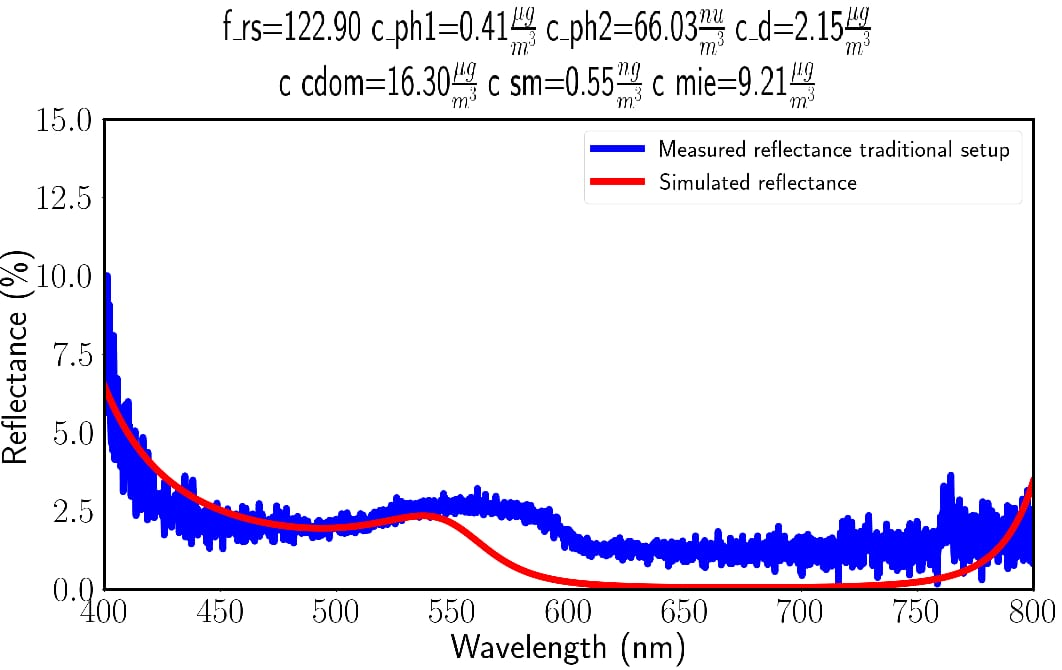
\includegraphics[scale=0.30]{./Figures/Simu_2.jpeg}
\caption{Simulation for .}
\end{figure}
\end{frame}

\begin{frame}
\frametitle{Simulations for MAZ\&-DOAS}
\begin{figure}
\centering
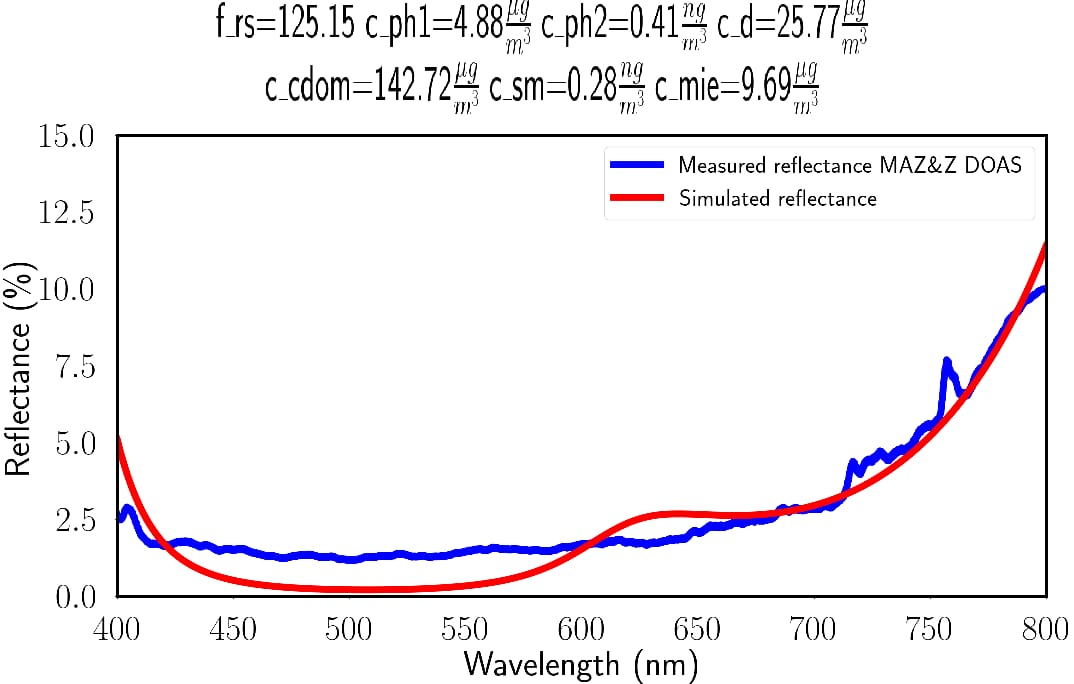
\includegraphics[scale=0.30]{./Figures/Simu_1.jpeg}
\caption{Simulation for .}
\end{figure}
\end{frame}

\section{Conclusions and acknowledgements}

\begin{frame}
\frametitle{Conclusions}
\begin{itemize}
\item Inversion of values for phytoplankton and CDOM in water
\item Simulation reproduced quite well the experimental measurements
\item MA\&Z-DOAS has potential as a low-cost platform for water quality measurements
\item Possibility for collaboration for massive analysis data in HPC calculations LARCAD
\end{itemize}
\end{frame}

\begin{frame}
\frametitle{Acknowledgements}
\begin{itemize}
\item Consejo Superior Universitario Centroamericano and the International Development Research Centre (CSUCA-IDRC) for partially funding this research under grants 50ES and 45CR
\item Consejo de Investigaciones Científicas de la Universidad de El Salvador (CIC-UES) by the partial funding of this work under the projects 05.31, 06.18, 09.19 and 09.20
\item Center for High Technology (CeNAT) in Costa Rica due to the computer time used in LARCAD to perform the computational calculations.
\end{itemize}
\end{frame}

\end{document}
